\documentclass{ximera}

\graphicspath{{./graphics/}}

\title{Lagrange Multipliers}
\begin{document}
\begin{abstract}
\end{abstract}
\maketitle

We've seen how we can optimize a function subject to a constraint using substitution, and we've seen that it can be very difficult to correctly handle the constraints! Fortunately, there is a tool that we can use to simplify this process. This tool is called ``Lagrange multipliers.''

\section*{Gradients}

Suppose we wish to optimize a function $f:\mathbb{R}^n\rightarrow\mathbb{R}$ subject to some constraint $g(\vec{x}) = C$, where $C$ is a constant, and $g:\mathbb{R}^n\rightarrow\mathbb{R}$ is a function. For now, we'll focus on the case $n=2$, so we have a function $f:\mathbb{R}^2\rightarrow\mathbb{R}$ and a constraint $g(x,y) = C$. The graph of $f$ will be a surface in $\mathbb{R}^3$, 

\begin{image}
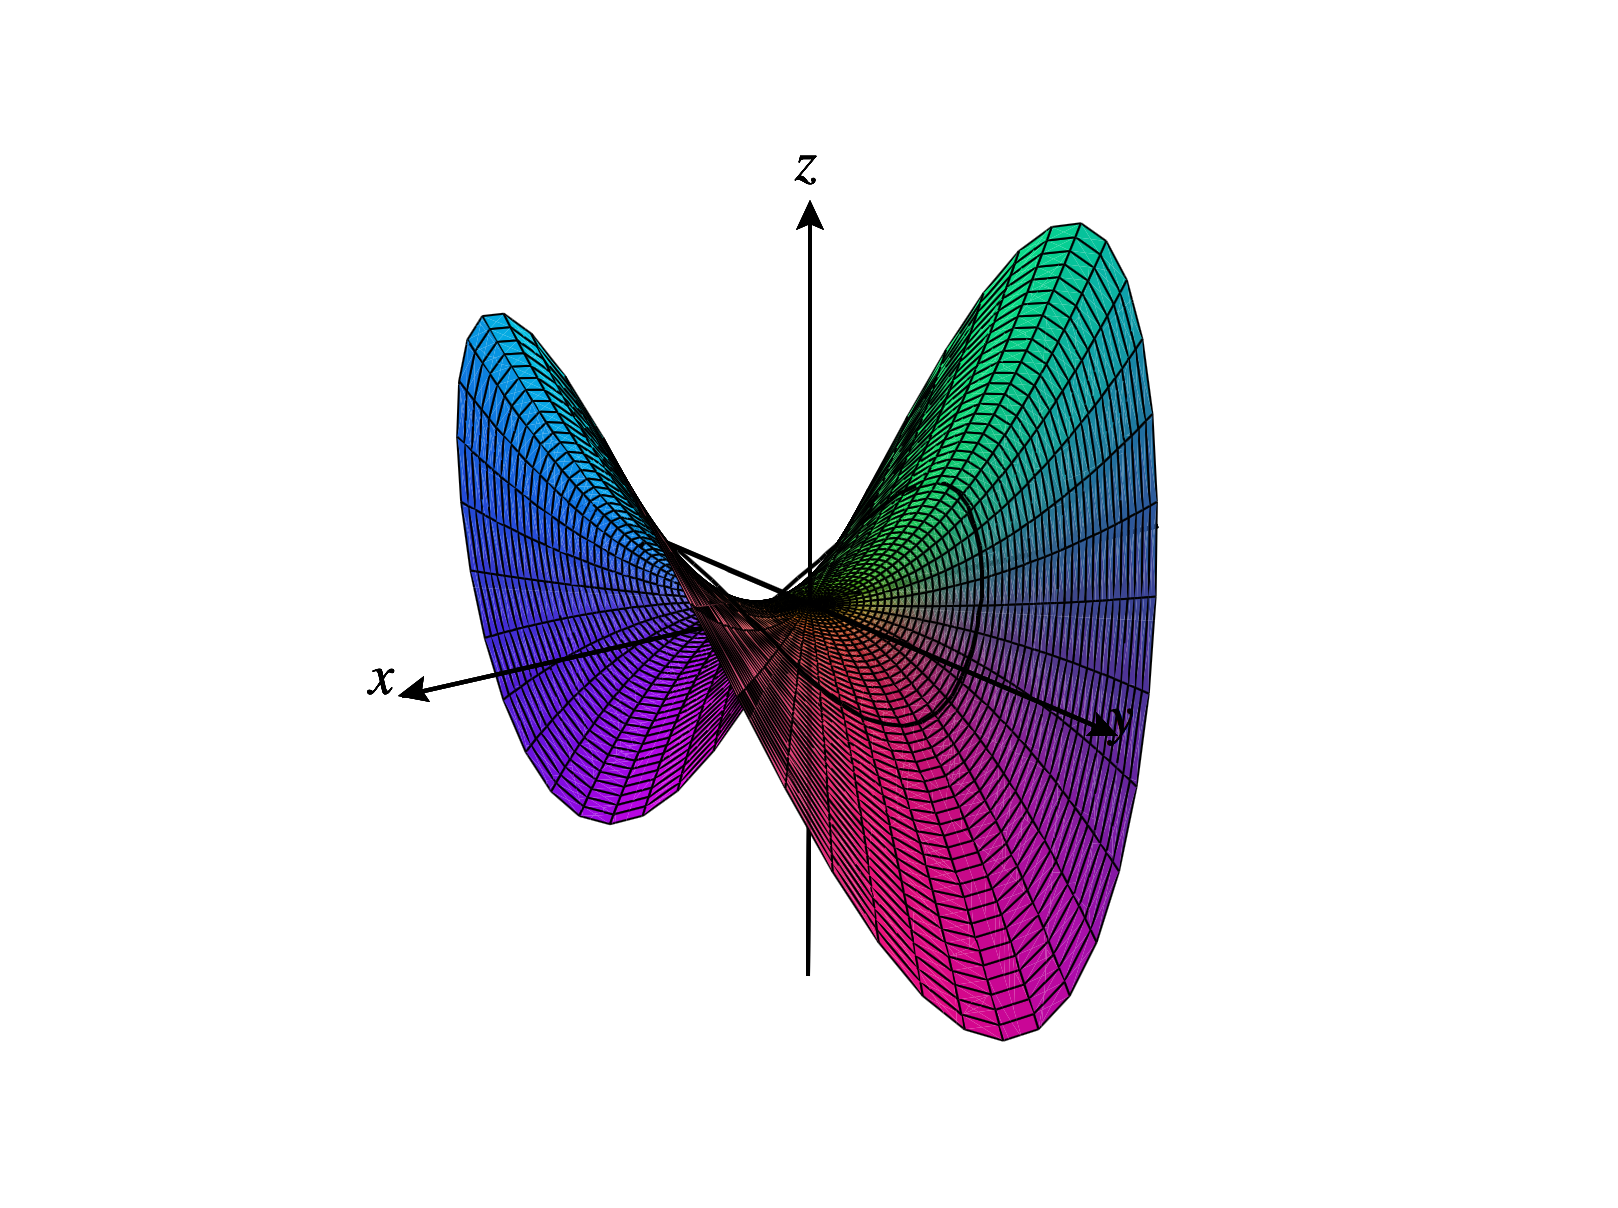
\includegraphics[width = \textwidth]{CalcPlot3D-surface}
\end{image}

and the graph of $g(x,y) = C$ is a curve in $\mathbb{R}^2$.

\begin{image}
\begin{tikzpicture}
\draw (0,0) circle (1);
\draw[<->] (-2,0) -- (2,0);
\node[anchor = west] at (2,0) {$x$};
\draw[<->] (0,-2) -- (0,2);
\node[anchor = south] at (0,2) {$y$};
\end{tikzpicture}
\end{image}

Now, suppose that the maximum value of $f(x,y)$ subject to the constraint $g(x,y)=C$ occurs at some point $(a,b)$. Suppose we parametrize the curve $g(x,y)=C$ as $\vec{x}(t)$, with $(a,b)=\vec{x}(t_0)$. We can view $g(x,y)=C$ as a level curve of the function $g(x,y)$, and then the gradient of $g(x,y)$ will always be perpendicular to the curve $g(x,y)=C$.

\begin{image}
\begin{tikzpicture}
\draw[<->] (-2,0) -- (2,0);
\node[anchor = west] at (2,0) {$x$};
\draw[<->] (0,-2) -- (0,2);
\node[anchor = south] at (0,2) {$y$};

\draw[color = purple] (0,0) circle (1);
\node[anchor = west] at (.7,-.8) {\color{purple} $g(x,y) = C$};
\draw[->, color = blue] (.707,.707) -- (1.2,1.2);
\node[anchor = west] at (1.2,1.2) {\color{blue} $\nabla g$};
\end{tikzpicture}
\end{image}

More precisely, for any point $(x,y) = \vec{x}(t)$ on the curve $g(x,y)=C$, we'll have $\nabla g(x,y)$ is perpendicular to $\vec{x}'(t)$. That is, $\nabla g(\vec{x}(t))\perp \vec{x}'(t)$ for all $t$.

\begin{image}
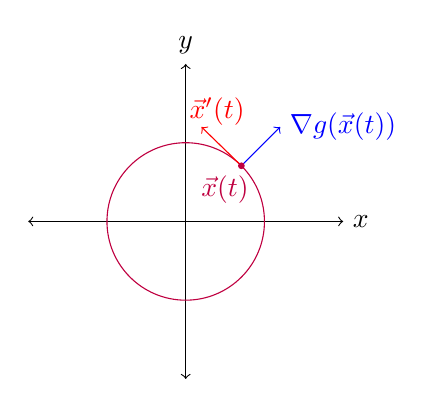
\begin{tikzpicture}
\draw[<->] (-2,0) -- (2,0);
\node[anchor = west] at (2,0) {$x$};
\draw[<->] (0,-2) -- (0,2);
\node[anchor = south] at (0,2) {$y$};


\draw[color = purple] (0,0) circle (1);
\draw[->, color = blue] (.707,.707) -- (1.2,1.2);
\node[anchor = west] at (1.2,1.2) {\color{blue} $\nabla g(\vec{x}(t))$};
\draw[->, color = red] (.707,.707) -- (.2,1.2);
\node[anchor = south] at (.4,1.1) {\color{red} $\vec{x}'(t)$};
\draw[color = purple, fill = purple] (.707,.707) circle (1pt);
\node[anchor = north] at (.5,.707) {\color{purple} $\vec{x}(t)$};
\end{tikzpicture}
\end{image}

Next, let's turn our attention back to $f$. If $f$ has an absolute maximum subject to $g(x,y)=C$, then $f(\vec{x}(t))$ has an absolute maximum at $t=t_0$. This means that $f(\vec{x}(t))$ has a critical point at $t=t_0$, so $\frac{d}{dt}f(\vec{x}(t))|_{t=t_0}=0$. Using the chain rule, we can rewrite this as
\[
\nabla f(\vec{x}(t_0))\cdot \vec{x}'(t)=0.
\]
So, both $\nabla f(a,b)$ and $\nabla g(a,b)$ are perpendicular to $\vec{x}'(t)$. Since we are considering vectors in $\mathbb{R}^2$, this means that $\nabla f(a,b)$ and $\nabla g(a,b)$ are parallel, so we can write
\[
\nabla f(a,b) = \lambda \nabla g(a,b)
\]
for some constant $\lambda$.

So, we can find candidate points for the absolute maximum (and similarly, the absolute minimum) of $f(x,y)$ subject to the constraint $g(x,y)=C$ by finding points where
\[
\nabla f(a,b) = \lambda \nabla g(a,b).
\]
This observation generalizes to $\mathbb{R}^n$.

\begin{proposition}
Consider $\mathcal{C}^1$ functions $f,g:\mathbb{R}^n\rightarrow\mathbb{R}$, and let $C$ be a constant. If $f$ has an absolute maximum or absolute minimum at $\vec{a}$ subject to the constraint $g(\vec{x}) = C$, then there exists some scalar $\lambda$ such that
\[
\nabla f(\vec{a}) = \lambda \nabla g(\vec{a}).
\]
The constant $\lambda$ is called a \emph{Lagrange Multiplier}.
\end{proposition}

We can leverage this theorem into a method for finding absolute extrema of a function subject to a constraint, which we call the \emph{method of Lagrange multipliers}.

To find the absolute extrema of a function $f(\vec{x})$ subject to a constraint $g(\vec{x})=C$:
\begin{enumerate}
\item Compute the gradients $\nabla f(\vec{x})$ and $\nabla g(\vec{x})$.
\item Solve the system of equations
\[\begin{cases}
\nabla f(\vec{x}) = \lambda \nabla g(\vec{x})\\
g(\vec{x}) = C
\end{cases}\]
for $\vec{x}$ and $\lambda$. 
\item The solutions to the system of equations in (2) are the critical points of $f(\vec{x})$ subject to $g(\vec{x}) = C$. Classify these critical points in order to determine the absolute extrema.

If $g(\vec{x})=C$ is compact, we can determine the absolute extrema by comparing the values of $f$ at the critical points. In this case, absolute extrema are guaranteed to exist by the Extreme Value Theorem.
\end{enumerate}

We'll see how this process works in a couple of examples. First, we repeating an optimization problem which was previously done with substitution.

\begin{example}
We'll find the absolute maximum and absolute minimum of $f(x,y) = x^2-y^2$ subject to the constraint $x^2+y^2=1$. Notice that $x^2+y^2=1$ is a compact region, so absolute extrema will exist.

If we let $g(x,y) = x^2+y^2$, our constraint is $g(x,y) = 1$.

Computing the gradients of $f$ and $g$, we have
\begin{align*}
\nabla f(x,y) &= \answer{(2x, -2y)},\\
\nabla g(x,y) &= \answer{(2x, 2y)}.
\end{align*}
Setting up the system of equations
\[\begin{cases}
\nabla f(\vec{x}) = \lambda \nabla g(\vec{x})\\
g(\vec{x}) = 1
\end{cases}, \]
we have
\begin{align*}
\nabla (2x,-2y) &= \lambda (2x, 2y)\\
x^2+y^2&=1\\
\end{align*}
We can rewrite this as a system of three equations,
\[\begin{cases}
2x=2\lambda x\\
2y=-2\lambda y\\
x^2 +y^2 =1
\end{cases}. \]

From the first equation, we have either $x=0$ or $\lambda =1$.

If $x=0$, the third equation gives us $y=\pm 1$. Thus, we obtain the critical points $(0,\pm 1)$.

If $\lambda =1$, the second equation gives us $y=0$. Then, the third equation gives us $x = \pm 1$. This gives us the critical points $(\pm 1, 0)$.

Since we know that $f$ will have an absolute maximum and minimum subject to our constraint, we will compare the values at the critical points to determine the absolute maximum and minimum.
\begin{align*}
f(0,-1) &= -1\\
f(0,1) &= -1\\
f(-1,0) &= 1\\
f(1,0) &=1
\end{align*}

We see that the absolute maximum of $f$ subject to our constraint is $1$, and this occurs at the points $(\pm 1, 0)$. The absolute minimum of $f$ subject to our constraint is $-1$, and this occurs at the points $(0,\pm 1)$. 
\end{example}

\begin{example}
Next, we'll attempt to optimize $f(x,y) = 12-x^2-y^2$ subject to the constraint $y^2=x+5$. Here, we'll need to be a bit more careful, since the curve defined by $y^2=x+5$ is not compact, as it is unbounded. 

\begin{image}
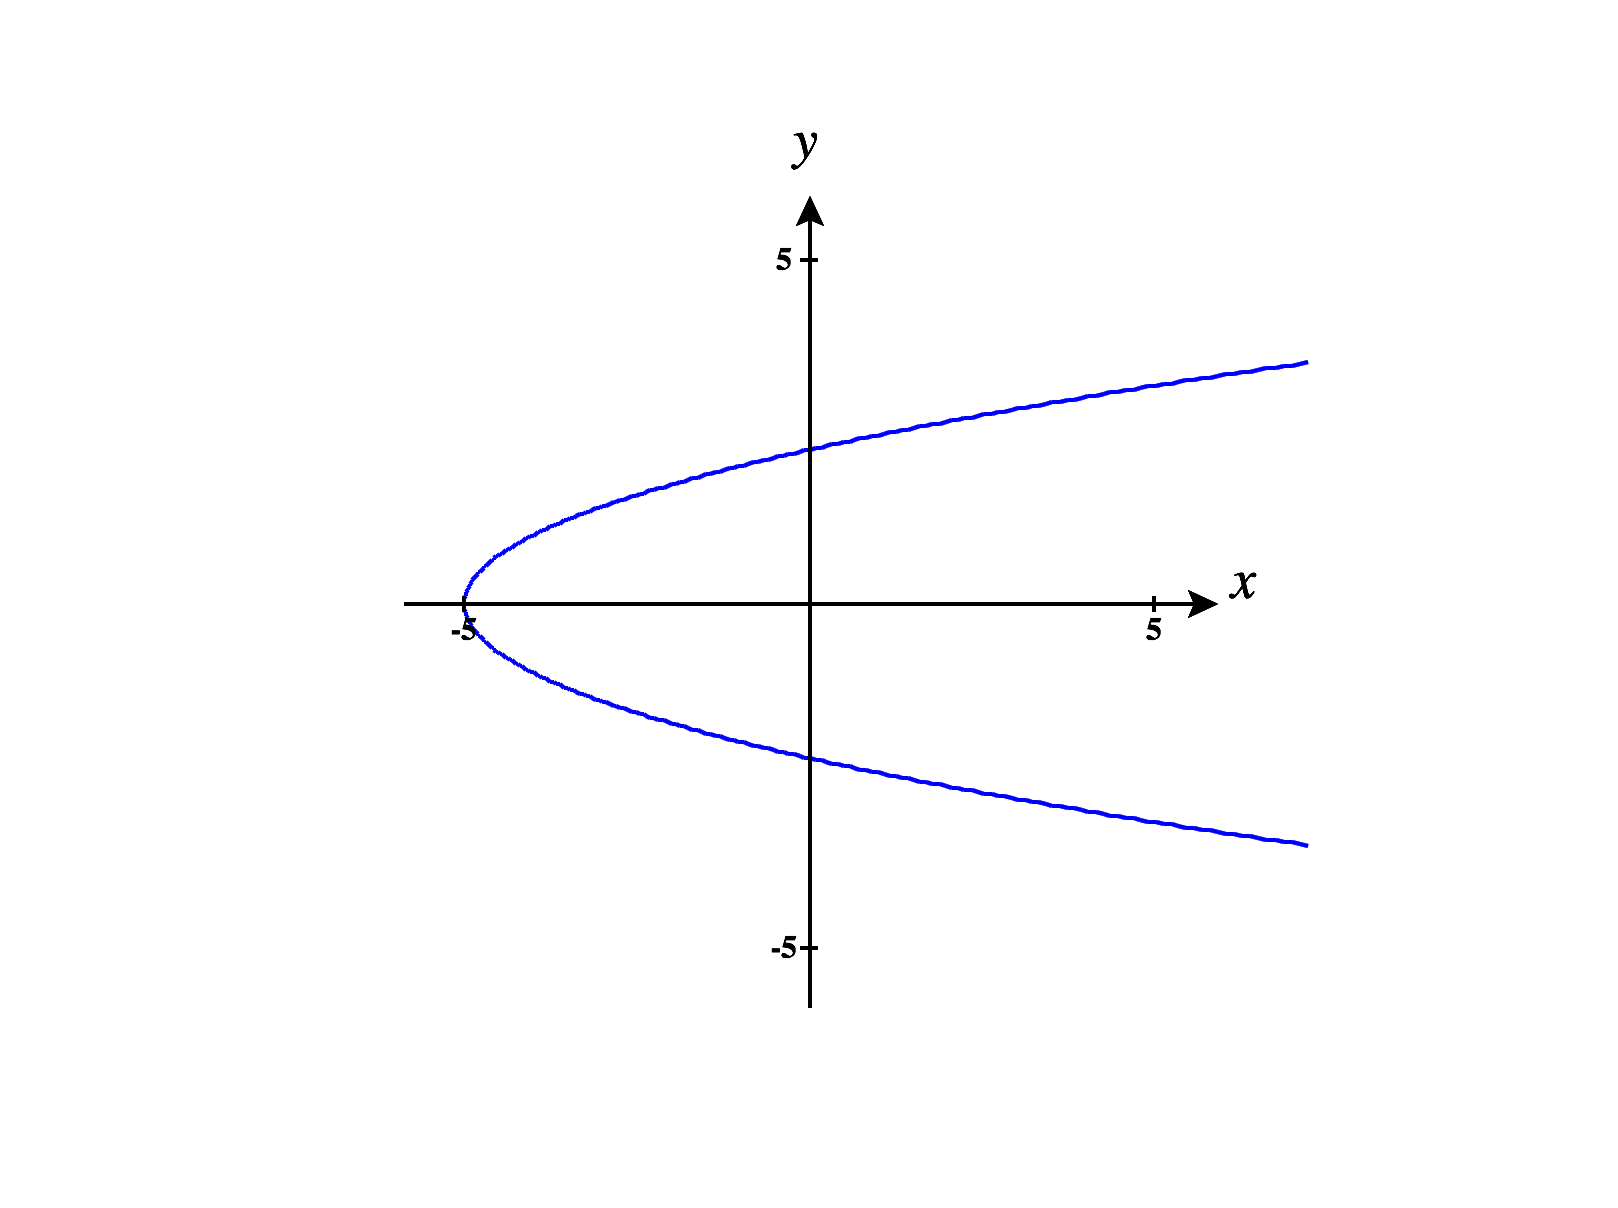
\includegraphics[width = \textwidth]{CalcPlot3D-parabola}
\end{image}

However, Lagrange multipliers will still be helpful for finding critical points. We can rewrite our constaint as $y^2-x=5$, and take $g(x,y) = y^2-x$. So, we are optimizing $f(x,y)$ subject to the constraint $g(x,y) = 5$.

We begin by finding the gradients of $f$ and $g$.
\begin{align*}
\nabla f(x,y) &= \answer{(-2x, -2y)}\\
\nabla g(x,y) &= \answer{(-1, 2y)}
\end{align*}
Next, we solve the system
\[\begin{cases}
\nabla f(\vec{x}) = \lambda \nabla g(\vec{x})\\
g(\vec{x}) = 5
\end{cases}, \]
which is
\[\begin{cases}
(-2x,-2y) = \lambda (-1,2y)\\
y^2-x= 5
\end{cases}. \]
We can rewrite this system as the three equations
\[\begin{cases}
-2x = -\lambda\\
-2y = 2\lambda y\\
y^2-x= 5
\end{cases}. \]
From the second equation, we have either $y=0$, or $\lambda =-1$.

If $y=0$, the third equation gives us $x=-5$. So, we have a critical point $(-5,0)$.

If $\lambda =-1$, the first equation gives us $x= -\frac{1}{2}$. Then the third equation gives us $y=\pm\frac{3}{\sqrt{2}}$. So, we have the critical points $\left(-\frac{1}{2}, \pm\frac{3}{\sqrt{2}}\right)$.

In this case, we can't determine the absolute maximum and absolute minimum by plugging in these points, since we aren't optimizing over a compact region.

However, looking at the graph of $f$ over the curve $g(x,y) = 5$, we can see that the absolute maximum occurs at the points $\left(-\frac{1}{2}, \pm\frac{3}{\sqrt{2}}\right)$. Although there is a local minimum at $(-5,0)$, this is not an absolute minimum, as there is no absolute minimum.

\begin{image}
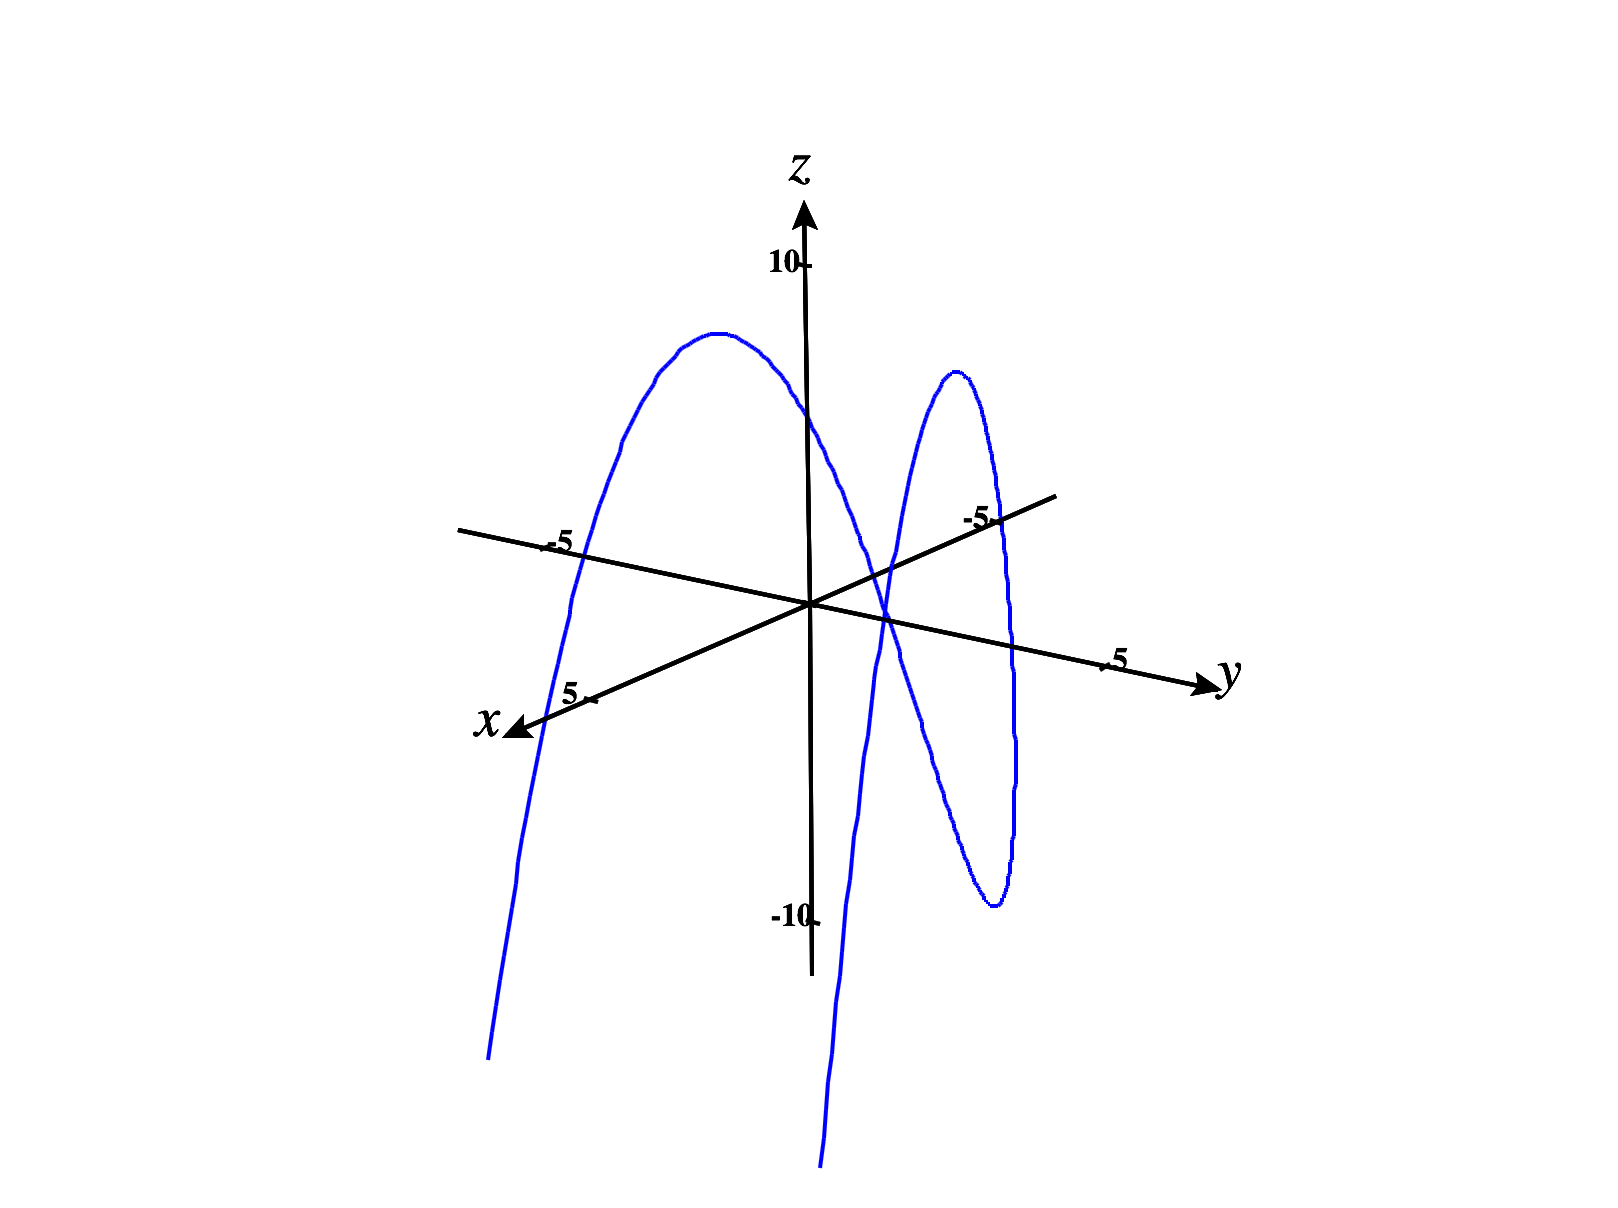
\includegraphics[width = \textwidth]{CalcPlot3D-constraint}
\end{image}

\end{example}

\end{document}